%% 
%% 報告書の LaTeX サンプル
%%	(version 4.9) 2020/06/03
%%

%\documentclass[bigbox]{jarticle}
\documentclass{jarticle}[11pt]
%\documentstyle[bigbox,fancybox]{jarticle}

% コマンドの定義
%
% コメントアウト用のコマンド
%   複数行にまたがる記述をまとめてコメントアウトする際に利用できる
%   \COMMENT{ .... } で .... の部分をコメントアウト
\newcommand{\COMMENT}[1]{}

% 以下は,表(srmmary.tex)で使用しているコマンド
\newcommand{\lw}[1]{\smash{\lower2.ex\hbox{#1}}}

% 図を参照するためのマクロ
\newcommand{\figref}[1]{\makebox{図~\ref{#1}}}

% 表を参照するためのマクロ
\newcommand{\tabref}[1]{\makebox{表~\ref{#1}}}

%% 使用しているパッケージ等があれば,宣言しておく
\usepackage{ascmac}
\usepackage{graphicx}

% 以下のパラメータは,見易いように適宜調整する.
\topmargin=-1cm
\textheight=24cm
\textwidth=15.5cm
\oddsidemargin=-.2cm
\evensidemargin=-.2cm

%% 報告書のタイトル,提出者,提出日等
%% これらのための専用の表紙を設ける必要はない.

%% 以下のタイトルは適切に変更すること
%% 「(の書き方)」も消すこと
\title{{\normalsize 情報工学実験A(ハードウェア)報告書(の書き方)}\\
(ここに適切な報告書のタイトルを記入のこと)
} 

%% 自分の学生番号と名前に変更すること.
\author{ 
  学生番号: 094305xx \\
  提出者: 渡邊 誠也 \\
  E-mail: nobuya@cs.okayama-u.ac.jp
}

%% 提出日を記載する.
\date{
  提出日: 2020年 6月xx日(?) \\ %% <-- 提出日を記載のこと
  締切日: 2020年 6月xx日(金)     %% <-- 締切日を記載のこと
}

\begin{document}
\maketitle

%%        1         2         3
%%2345678901234567890123456789012345678
%% (参考)
%% Emacs等のエディタでは通常,横に全角文字を40文字(半角で80文字)表示
%% できるため,このサンプルファイルのテキストは各行を34〜38文字程度に収まる
%% ように適宜改行を入れている.
%% テキスト中に改行をいれていても,LaTeXで整形後にその改行は出力されない.
%% 適切に改行をいれておくほうが,テキストの編集をしやすいため,こうしている.
%% 
%% 改行の箇所は,文章の編集しやすさを考慮して,可能な限り句読点の箇所や
%% 文章,文節の区切りでいれている.
%% Emacsでは 
%%   C-a ....... 行頭にカーソルを移動
%%   C-k C-k ... カーソルから行末までをコピーして削除(カット)
%%   C-y ....... カーソル位置にコピーしたテキストをはき出す(ヤンク).
%% で編集できるため,文章の区切りのよい箇所で改行を入れて別の行に記述して
%% おくほうが編集を容易に行うことができる.
%% 
%% マウスオペレーションで編集する人には関係ないかもしれないが...
%% 

\begin{abstract}
(ここに報告書の概要を簡潔にまとめる.
本文中にある文章をピックアップしつなげてまとめることで作成する.
特に「おわりに」にある文章が活用できる場合が多い.)

本稿では,情報工学実験A(ハードウェア)プロセッサ設計実験の報告書の
書き方について説明する.
報告書執筆における基本的な注意点について説明する.
さらに,報告書の作成と提出について簡単に述べる.
この文書の\LaTeX ソースを読むことで,\LaTeX を使った報告書の執筆について
スキルを得ることを期待する.
\end{abstract}


\section{はじめに}

報告書の最初の節(ここでは「{\gt はじめに}」というタイトルとしている)では,
実験の背景と目的,および,本報告書の構成について述べる.
報告書の構成は,各自の判断で分かりやすい構成にすればよい.
このサンプルでは,{\bf 1} 〜 {\bf 4} 節の構成をとっているが,
報告事項によって適宜変更する.
各節では小節(subsection)を設けるなどして,わかり易い構成をとって欲しい.
%% パラグラフを変える場合,次の行のように空行を1行以上入れればよい.

以下に,かなり省略してはいるが,「{\gt はじめに}」の記述例を示す.
節(section)や小節(subsection)等の参照には,
\verb|\ref{ラベル名}|といった記述を用いる.
ラベルの定義は,本ドキュメントのソースの見ればわかるだろう.

% パラグラフの冒頭で段下げをしたくない場合,下のように \noindent と書く
\noindent
【記述例】

本実験の目的は,.... .... ..... .... .... .... である.
本報告書では,.... について報告する.
% 次の行は,参考文献の引用例.〈文献のラベル〉を \cite{} で括る.
情報工学実験テキスト \cite{bib:実験テキスト} の第1章から第3章の
.... .... .... .... .... を報告する.

本報告書の構成は次のとおりである.
まず 
{\bf \ref{sec:報告書執筆における注意点}} にて.... .... .... .... .... 
について述べる.
{\bf \ref{sec:報告書の作成と提出}}では,.... .... .... .... .... .... 
.... .... する.
最後に {\bf \ref{sec:おわりに}} で,本報告のまとめと
.... .... を述べる.

\section{報告書執筆における注意点}
\label{sec:報告書執筆における注意点}

ここでは,執筆上の注意点について述べる.

\subsection{報告内容に関する事項}
実験レポートの報告内容に関する注意事項は次のとおりである.
\begin{enumerate}
\item 自分で文章を組み立てること.
テキストや参考にした文献やウェブページの文章を,
一言一句をそのままコピー\&ペーストしたのでは,
著作権の問題(盗作)があるばかりか,自分のためにもまったく意味がない.
参考にした文献で述べられていることを文中で引用する場合は,
末尾の参考文献にその文献を挙げ,本文中では文献番号を付加し,
他の文献からの引用であることを明確にすること.
例えば,
\begin{quote}
高速化を実現するために,イソテル社のプロセッサでもこの方式を
採用している\cite{bib:超高速プロセッサ}.
\end{quote}
というように,参考文献を引用する.

自分自身が記述してある内容を{\gt よく理解した上で自分の言葉で表現する}ように
努めて欲しい.
その際,事実を述べているのか,自分の意見や考えなのか,
他人の考えや意見なのかを明確に区別して書くように心がけて欲しい.

ただし,ここで言う「自分の言葉」というのは,日常,会話をする際に
使っている言葉ではなく,報告書の文章として適切な言葉のことである.
{\gt 口語体の文章は,報告書に用いる文章としては不適切}である点に
注意して欲しい.

\item 他人が読んで理解できるようにすること.
「報告書を読むのは担当教員だけだろうから,このことは担当教員も
知っているだろうからこの部分だけ述べることにしよう」といった
考えで報告書を書かないこと.
第三者が報告書のみで内容を把握できるように書くように努めて欲しい.
例えば,「課題$x$を行なった」とある場合,「課題$x$」はどういった
内容なのかを{\gt 簡潔にまとめて}報告書に記載しておくべきである.

\item 結果報告だけの内容にならないこと.
得られた結果に対しては,その結果が妥当な結果なのかを考察するべきである.
また自分で見い出した問題点や,その問題点を解決するまでに考えたこと等を
述べるべきである.

例えば,「課題$x$ を行ない,正しく動いた.」といった記述だけでは,
不十分である.
上の 2. とも関連するが,「課題$x$」は何なのか,「正しい」とは何をもって
正しいと言えるのかをきちんと正確に記述する必要がある.

また,「課題$y$ では,図$z$に示すFSL記述を作成した.(おわり)」といった
記述も不十分である.
課題の意図を理解し,そのFSL記述を作成するまでに考えたこと,
FSL記述の説明等を行なうべきである.
逆に,やみくもにすべてを説明していたのでは,
焦点が定まらず分かりにくくなることがあるので注意が必要である.
その図や説明で主張したいことを伝えることができるように工夫して欲しい.
\end{enumerate}

\subsection{体裁に関すること}

その他の注意事項(体裁に関すること)としては,次の事項が挙げられる.
%% 以下は enumerate 環境の使用例
\begin{enumerate}
\item 「〜です.」「〜します.」といった {\gt ですます調} で書かない.

\item 句読点は,「.」「,」を用いる
%技術文書では「。」や「、」はあまり用いられない
\footnote{例えば,情報処理学会,電子情報通信学会の和文の論文誌では,
句読点は「.」と「,」を用いている.}.
\verb|~/.emacs| ファイルに次の式を記述をしておけば,デフォルトの
句読点が「.」および「,」となる.
%; 以前の設定
%;(setq use-kuten-for-period nil) ;; nil の場合 「.」,t の場合「。」
%;(setq use-touten-for-comma nil) ;; nil の場合 「,」,t の場合「、」
%
% コード片などの比較的短いコード等を本文の中に入れたい場合,
% 下記のように「quote環境」と「verbatim環境」を用いるとよい.
\begin{quote}
\begin{verbatim}
;; 2バイト文字の句読点設定 
(setq its-hira-period ".") ;; 「.」は全角
(setq its-hira-comma  ",") ;; 「,」は全角
\end{verbatim}
\end{quote}
上記設定をしていない場合に「.」および「,」をタイプする場合,
日本語モードでそれぞれ\verb|Z-.|(大文字のZをタイプ後,ピリオド(.)をタイプ),
\verb|Z-,|(大文字のZをタイプ後,カンマ(,)をタイプ)を入力する.

\item \TeX の \verb|verbatim|環境の乱用は避ける.
しばしば,報告書全体を \verb|verbatim|環境にて書いている学生が見受けられる.
そのような書き方では \TeX で美しい文書が作成できる機能を十分に
利用できていないことになる(すなわち,レポート点の減点になりうる).
また,次以降に挙げる箇条書きやフォントの切替え等もできない.

\item 箇条書きや列挙を活用する.
実験報告書は基本的に,文章主体で書くべきものであるが,
文章だけでだらだらと書いていたのでは分かりにくい場合もある.
箇条書き(itemize)や列挙(enumerate)等を用いることでわかり易くなる場合には
積極的に利用することを推奨する.

\item フォントを適切に選択する.
例えば,強調したい単語は,{\gt ゴシック体}や{\gt \bf bold体}にするとか,
プログラムリストや結果出力は,タイプライタフェイス
(\verb|typewriter face|) のフォントで書くといったようにフォントを適切に使用するとわかり易い.プログラムコードなどには,タイプライタフェイスのフォント(\verb|this uses typewriter face fonts|)を用いる.

数式は,\LaTeX の数式モードを利用することで,
適切な数式用のフォントを使う.
このサンプルでは,適切なフォントを利用している.

\item 図や表には,図番号あるいは表番号とタイトルをつける.
また図や表を掲載する場合には,本文中でそれらの図番号あるいは表番号を
参照して説明をすること.本文にて言及されない図や表は掲載しない.

\item 長いソースリストや結果の記載は,付録を活用する.
(なお,本当にそのソースリストや結果の掲載が必要なのかよく考えること).
その際,図や表と同様,本文中から参照して簡単に説明すること.

\item 不要な改行や,改ページを行わないこと.パラグラフ(段落)は,
TeXのソースで空行を入れると適切に,別の段落として整形される.
本文中では,強制改行の \verb|\\| を使う必要なほとんどないはずである.
(表などでは必要である).

\end{enumerate}

ここでは,例として itemize環境の使い方を知らない人がよく書く
verbatim環境を用いた列挙の記述例を
\figref{fig:verbatim環境による列挙の記述例}に示す.
%
\begin{figure}[tb]
\begin{center}
\begin{quote}
\verb|\begin{verbatim}| \\
\verb|・ 最初の項目| \\
\verb|・ 次の項目| \\
\verb|・ 3番目の項目| \\
\verb|・ 最後の項目| \\
\verb|\end{verbatim}|
\end{quote}
\caption{verbatim環境による列挙の記述例}
\label{fig:verbatim環境による列挙の記述例}
\end{center}
\end{figure}
%
\begin{figure}[tb]
\begin{quote}
\begin{verbatim}
\begin{itemize}
  \item 最初の項目
  \item 次の項目
  \item 3番目の項目
  \item 最後の項目
\end{itemize}
\end{verbatim}
\end{quote}
\caption{itemize環境による列挙の記述例}
\label{fig:itemize環境による列挙の記述例}
\end{figure}
%
\figref{fig:verbatim環境による列挙の記述例}に示すコードからは,
\LaTeX により次のように整形される.
%
\begin{quote}
\begin{verbatim}
・ 最初の項目
・ 次の項目
・ 3番目の項目
・ 最後の項目
\end{verbatim}
\end{quote}

\figref{fig:verbatim環境による列挙の記述例}に示した記述は,
\LaTeX では\figref{fig:itemize環境による列挙の記述例}に示す記述のように
itemize環境を用いた記述にするべきである.
\figref{fig:itemize環境による列挙の記述例}に示すソースコードからは,
\LaTeX により次のように整形される.
\begin{quote}
\begin{itemize}
  \item 最初の項目
  \item 次の項目
  \item 3番目の項目
  \item 最後の項目
\end{itemize}
\end{quote}

各項目に番号を振りたい場合,
\verb|itemize|環境の代わりに\verb|enumerate|環境を利用するとよい.
\figref{fig:verbatim環境による列挙の記述例}に示した記述を
\verb|enumerate|環境で記述した際には次のように整形される.
\begin{quote}
\begin{enumerate}
  \item 最初の項目
  \item 次の項目
  \item 3番目の項目
  \item 最後の項目
\end{enumerate}
\end{quote}

最初から完全な報告書は要求しないが,徐々に改善していくように
努力してもらいたい.
4年生で研究室配属されると所属研究室の教員から特別研究の指導を受け,
最終的に特別研究報告書にまとめる際に事細かい指導を受けることになるが,
日頃のレポートや報告書作成においても自分自身でよりよい報告書と
なるように取り組んでいくことを推奨する.

なお,本ドキュメントの \LaTeX ソースを公開するので,
報告書を作成する際の参考にして頂きたい.
この文書自体にはあらわれていないが,ソース内にコメント等を追加してあるので
参照されたい.

%提出する前に,内容のチェック,体裁やフォントのチェック等を
%しっかりと行なうこと.

\section{報告書の作成と提出}
\label{sec:報告書の作成と提出}
\LaTeX で作成した実験報告書は,
PDFファイルに変換して所定の場所へ提出する.
提出方法等に関しては,別途,指示があるのでそちらにしたがうこと.

\subsection{報告書の作成}
% 2020年度は,実験用サーバあるいは自宅PCの環境で行う.
%報告書は,演習室計算機上の \LaTeX で作成する.
報告書は,実験用サーバの \LaTeX あるいは,自宅PCの環境で作成する.
報告内容や執筆上の注意点は,
{\bf \ref{sec:報告書執筆における注意点}}で述べたとおりである.
エディタ(Emacs等)で報告書ファイルを記述し,\LaTeX で整形する.
\LaTeX の使い方については,情報工学実験の範囲ではないので
ここでは説明しない.
適宜,プログラミング演習で習ったことを復習しておくこと.

DVIファイルをPDFファイルへ変換する際には,
\verb|dvipdfmx| コマンドを用いる.
\LaTeX で生成した DVI ファイル \verb|report.dvi| を
\verb|report.pdf| というファイル名の PDF ファイルに変換する例を
\figref{fig:DVIファイルの作成例}に示す.
\begin{figure}[htb]
{\small
\begin{quote}
\begin{verbatim}
nobuya@edu006[304]% platex report.tex
This is pTeX, Version p2.1.11, based on TeX, Version 3.14159 (EUC) (Web2C 7.3.1)(report.tex
pLaTeX2e <2000/11/03>+0 (based on LaTeX2e <2001/06/01> patch level 0)
(/usr/share/texmf/ptex/platex/base/jarticle.cls
Document Class: jarticle 1999/05/18 v1.1q Standard pLaTeX class
(/usr/share/texmf/ptex/platex/base/jsize10.clo))
(/usr/share/texmf/ptex/platex/base/ascmac.sty
(/usr/share/texmf/ptex/platex/base/tascmac.sty))
(/usr/share/texmf/tex/latex/graphics/graphicx.sty
(/usr/share/texmf/tex/latex/graphics/keyval.sty)
(/usr/share/texmf/tex/latex/graphics/graphics.sty
(/usr/share/texmf/tex/latex/graphics/trig.sty)
(/usr/share/texmf/tex/latex/config/graphics.cfg)
(/usr/share/texmf/tex/latex/graphics/dvips.def))) (report.aux) [1] [2] [3]
[4] (alu4.sfl.tex) [5] [6] <count4_gtkwave.eps> [7] (report.aux) )
Output written on report.dvi (7 pages, 23196 bytes).
Transcript written on report.log.
nobuya@edu006[305]%
\end{verbatim}
\end{quote}
} % small
\caption{DVIファイルの作成例}
\label{fig:DVIファイルの作成例}
\end{figure}
作成した PDFファイルがプレビューア (\verb|xpdf|,\verb|acroread|等)で
読めるかを提出する前に確認することを忘れないで欲しい.
2020年度は,演習室PCを利用しないため,生成したPDFファイルを手元のPCに
コピーしてプレビューアは自分の手元のPCで行う必要がある.


\section{おわりに}
\label{sec:おわりに}
最後の節では,本報告書のまとめを述べる.
どういったことを報告したのか,目的は達成できたか,どういう成果があったか,
どういうことが分かったのか,不十分な点や課題事項は何かを簡潔にまとめる.
% 例えば,実験テキスト\cite{bib:実験テキスト}の章末にあるチェック項目の
% 事項が達成できたかを示せばよいだろう.

なお,この「おわりに」に書かれていることは,基本的に「おわりに」に至るまでの
本文中に書かれていることであるべきである.
つまり,ここには本文中で書かれていない新たなことを書くことは避けるべきである.

\noindent
【記述例】

本報告書では,.... .... .... .... .... .... .... について報告した.
本実験テーマの目的である(1) ....,(2) ... $\cdots$ ($n$) ... は,
それぞれ達成できた.
また,.... .... により, .... .... であることがわかった.
%% 今後の課題としては .... .... がある.

%%
%% 報告書の中で参照した参考文献があれば,次の形式にて記述する.
%% 参照している箇所では,\bib{ラベル} にて参照する.
%% 参考にしたウェブページ等があれば,URL等を書いておく.
%% 本文中で参照していない文献はここに挙げないこと.
\begin{thebibliography}{9}
\bibitem{参考文献} 著者名,文献のタイトル,(もしあればページ,),
出版社,出版年.
%% 以下,記述例 (次の文献は「はじめに」で引用している.)
\bibitem{bib:実験テキスト} % 架空のテキストです.
渡邊誠也,ハードウェア記述言語を用いたマイクロプロセッサの設計,
情報工学実験テキスト,岡山大学工学部情報工学科,2003.
\bibitem{bib:超高速プロセッサ} % 架空のURLです.
イソテル社の超高速プロセッサ, http://www.isotel.co.jp/high-speed-processor/.
\end{thebibliography}

%%
%% 報告書本文に記載できないが,情報として必要なものがあれば
%% 付録にて記載する.

%% 必要なら改ページ
\newpage
\appendix

\noindent
{\Large \gt 付録}

報告書本体部分に掲載するとわかりにくくなるものは,付録に掲載する.
例えば,出力結果全体やFSL記述のリストなどである.
本文中に掲載したほうが,分かりやすい場合は本文中に掲載すべきであり,
その場合でも掲載は説明に必要な最小限になるように努めるべきである.

\section{8ビットALUのFSL記述}
\label{appsec:8ビットALUのFSL記述}

\begin{figure}[hbtp]
\begin{center}
% 外部ファイルの読み込み
% This file generated by Src2tex.scala
%
\begin{quote}
\begin{tabular}{r|l}
    1 & \verb|/* (alu8.fsl) */| \\ [-3pt]
    2 & \verb|module alu8 {| \\ [-3pt]
    3 & \verb|  input         a: Bit(8)| \\ [-3pt]
    4 & \verb|  input         b: Bit(8)| \\ [-3pt]
    5 & \verb|  output      out: Bit(8)| \\ [-3pt]
    6 & \verb|  output overflow: Bit(1)| \\ [-3pt]
    7 & \verb|  output     zero: Bit(1)| \\ [-3pt]
    8 & \verb|| \\ [-3pt]
    9 & \verb|  val adder = new add8 // module instatiation| \\ [-3pt]
   10 & \verb|| \\ [-3pt]
   11 & \verb|  private def zero_check(): Unit = {| \\ [-3pt]
   12 & \verb|    zero = if (out == 0x00) 0b1 else 0b0| \\ [-3pt]
   13 & \verb|  }| \\ [-3pt]
   14 & \verb|  def op_add(a, b): Unit = {| \\ [-3pt]
   15 & \verb|    out = adder.add(a, b, 0b0).sum| \\ [-3pt]
   16 & \verb+    overflow = ((~a(7) & ~b(7) &  out(7)) |+ \\ [-3pt]
   17 & \verb|                ( a(7) &  b(7) & ~out(7)))| \\ [-3pt]
   18 & \verb|    zero_check()| \\ [-3pt]
   19 & \verb|  }| \\ [-3pt]
   20 & \verb|  def op_sub(a, b): Unit = {| \\ [-3pt]
   21 & \verb|    out = adder.add(a, ~b, 0b1).sum| \\ [-3pt]
   22 & \verb+    overflow = ((~a(7) &  b(7) &  out(7)) |+ \\ [-3pt]
   23 & \verb|                ( a(7) & ~b(7) & ~out(7)))| \\ [-3pt]
   24 & \verb|    zero_check()| \\ [-3pt]
   25 & \verb|  }| \\ [-3pt]
   26 & \verb|  def op_and(a, b): Unit = {| \\ [-3pt]
   27 & \verb|    out = a & b| \\ [-3pt]
   28 & \verb|    overflow = 0b0| \\ [-3pt]
   29 & \verb|    zero_check()| \\ [-3pt]
   30 & \verb|  }| \\ [-3pt]
   31 & \verb|  def op_or(a, b): Unit = {| \\ [-3pt]
   32 & \verb+    out = a | b+ \\ [-3pt]
   33 & \verb|    overflow = 0b0| \\ [-3pt]
   34 & \verb|    zero_check()| \\ [-3pt]
   35 & \verb|  }| \\ [-3pt]
   36 & \verb|  def op_xor(a, b): Unit = {| \\ [-3pt]
   37 & \verb|    out = a ^ b| \\ [-3pt]
   38 & \verb|    overflow = 0b0| \\ [-3pt]
   39 & \verb|    zero_check()| \\ [-3pt]
   40 & \verb|  }| \\ [-3pt]
   41 & \verb|  def op_nor(a, b): Unit = {| \\ [-3pt]
   42 & \verb+    out = ~(a | b)+ \\ [-3pt]
   43 & \verb|    overflow = 0b0| \\ [-3pt]
   44 & \verb|    zero_check()| \\ [-3pt]
   45 & \verb|  }| \\ [-3pt]
   46 & \verb|} // module alu8| \\ [-3pt]
   47 & \verb|/* End of file (alu8.fsl) */| \\ [-3pt]
\end{tabular}
\end{quote}
% End 

\caption{8ビットALUのFSL記述}
\label{fig:8ビットALUのFSL記述}
\end{center}
\end{figure}

\figref{fig:8ビットALUのFSL記述}に8ビットALUのFSL記述を示す.
\figref{fig:8ビットALUのFSL記述}の11行目から13行目で内部関数
\verb|zero_check| を定義している.
このモジュールで定義されている入力関数では,出力\verb|out|を求め,
内部関数\verb|zero_check| を起動し,出力\verb|out|の値が
ゼロかゼロでないかを判定し,出力\verb|zero|の値を求めている.

\section{表の例}

表の例を\tabref{tab:FPGAへの論理合成等で得られた諸量のまとめ}〜
%\tabref{tab:マイクロプロセッサp16の設計状況}
\tabref{tab:目標達成度と自己評価}に示す.
なお,表の見出し(表題)は表の上に配置する.
一方,図の見出しは図の下に配置することに注意のこと.
FSL記述等のソースリストは図扱いとする.
%\footnote{表の見出し(表題)は,表の上に置く.一方,図の見出しは図の
%下に置く.}.

表を参照する際には,単に表を掲載するだけではなく,
「表~\ref{tab:FPGAへの論理合成等で得られた諸量のまとめ}にFPGAへの
論理合成,配置配線,および静的タイミング解析で得られた諸量をまとめた結果を
示す.
ターゲットとしたFPGAデバイスとそのリソース量を
表~\ref{tab:ターゲットFPGAデバイスとそのリソース量}に示す.」
といった文章にて,
参照している「表」が何を示しているのかを本文中で説明した後に,
その詳細に関する説明が必要である.
本文中から参照されない図表は,載せてはいけない.

また,表に無駄に線(縦線,横線)を入れないこと.
項目の区切りの部分など必要最低限に留めるようにすること.

% 別ファイル(summary.tex)に記述して読み込む場合
%\begin{table}[tb]
\caption{FPGAへの論理合成等で得られた諸量のまとめ}
\label{tab:FPGAへの論理合成等で得られた諸量のまとめ}
\begin{center}
% 表が大きいので,small サイズのフォントを利用
{\small
\begin{tabular}{l|ccccc}
\hline
\hline
\lw{モジュール} &
\multicolumn{2}{c}{最大動作周波数 Fmax} & \lw{LE数 (使用率)} & 
\lw{CF数 (使用率)} & \lw{レジスタ数 (使用率)}  \\
& 85 $^\circ$C Model & 0 $^\circ$C Model & & &  \\
\hline
プロセッサ \verb|p16m1| & 12.34 & 23.45 & 
    12,345 (2\%) & 1,111 (1\%)&  2,222 (2 \%) \\
プロセッサ \verb|p16m2| & & & & & \\
プロセッサ \verb|p16p1| & & & & & \\
\hline
\multicolumn{6}{r}{(Fmax の単位は MHz)}
\end{tabular}
}
\end{center}
\end{table}

\begin{table}[tb]
\caption{ターゲットFPGAデバイスとそのリソース量}
\label{tab:ターゲットFPGAデバイスとそのリソース量}
\begin{center}
\begin{tabular}{l|r}
\hline \hline
ターゲットデバイス & Intel Cyclone IV E (EP4CE115F29C7) \\
Logic Element (LE)数 & 114,480 \\
レジスタ数 & 114,480 \\
メモリ容量 (ビット) & 4,981,312\\
9ビット乗算器 & 432 \\
\hline
\end{tabular}
\end{center}
\end{table}


% このファイルに直接記述する場合

%
% 合成結果で得られた諸量のまとめの表は,Webの登録ページにて
% LaTeXの表ソースを生成することもできるので,活用されたい
% (注意: 2020年度にはこの機能は提供されていません)
%
\begin{table}[tb]
\caption{FPGAへの論理合成等で得られた諸量のまとめ}
\label{tab:FPGAへの論理合成等で得られた諸量のまとめ}
\begin{center}
% 表が大きいので,small サイズのフォントを利用
{\small
\begin{tabular}{l|ccccc}
\hline
\hline
\lw{モジュール} &
\multicolumn{2}{c}{最大動作周波数 Fmax} & \lw{LE数 (使用率)} & 
\lw{CF数 (使用率)} & \lw{レジスタ数 (使用率)}  \\
& 85 $^\circ$C Model & 0 $^\circ$C Model & & &  \\
\hline
プロセッサ \verb|p16m1| & 12.34 & 23.45 & 
    12,345 (2\%) & 1,111 (1\%)&  2,222 (2 \%) \\
プロセッサ \verb|p16m2| & & & & & \\
プロセッサ \verb|p16p1| & & & & & \\
\hline
\multicolumn{6}{r}{(Fmax の単位は MHz)}
\end{tabular}
}
\end{center}
\end{table}

\begin{table}[tb]
\caption{ターゲットFPGAデバイスとそのリソース量}
\label{tab:ターゲットFPGAデバイスとそのリソース量}
\begin{center}
\begin{tabular}{l|r}
\hline \hline
ターゲットデバイス & Intel Cyclone IV E (EP4CE115F29C7) \\
Logic Element (LE)数 & 114,480 \\
レジスタ数 & 114,480 \\
メモリ容量 (ビット) & 4,981,312\\
9ビット乗算器 & 432 \\
\hline
\end{tabular}
\end{center}
\end{table}

% 別ファイル(status.tex)に記述して読み込む場合
%\begin{table}[tb]
\caption{プログラミング課題と設計課題の実施状況}
\label{tab:プログラミング課題と設計課題の実施状況}
\begin{center}
{\small
\begin{tabular}{rll|l}
\hline
\hline
\multicolumn{3}{c|}{課題} & 状況 \\
\hline
\multicolumn{3}{l|}{(プログラミング課題)} & \\
1. & \multicolumn{2}{l|}{【プログラミング課題1】$N$個の語の加算 } & (2)完了 \\
2. & \multicolumn{2}{l|}{【プログラミング課題2】$N$語のメモリコピー} & (0)未実施 \\
3. & \multicolumn{2}{l|}{【プログラミング課題3】乗算} & (2)完了 \\
\multicolumn{3}{l|}{(設計課題2)} & \\
4. & 【設計課題2-1】32ビット加算器   & \verb|add32|          & (0)未実施 \\
5. & 【設計課題2-2】32ビットALU      & \verb|alu32|          & (1)設計中 \\
6. & 【設計課題2-3】32ビットシフタ   & \verb|shift32|        & (2)設計完了 \\
\multicolumn{3}{l|}{(発展課題2)} & \\
7. & 【発展課題2-1】32ビット整数乗算器 & \verb|mult32|       & (0)未実施 \\
8. & 【発展課題2-1】32ビット整数除算器 & \verb|div32|        & (0)未実施 \\
\multicolumn{3}{l|}{(設計課題3)} & \\
9. & 【設計課題3-1】レジスタファイル & \verb|regs32x32|      & (0)未実施 \\
10. & 【設計課題3-2】実行ユニット     & \verb|p32ExecUnit|    & (0)未実施 \\
11. & 【設計課題3-3】デコードユニット & \verb|p32DecodeUnit|  & (0)未実施 \\
\multicolumn{3}{l|}{(設計課題4)} & \\
12. & 【設計課題4-1】プロセッサ      & \verb|p32m1|          & (0)未実施 \\
13. & 【設計課題4-2】プロセッサ      & \verb|p32m2|          & (0)未実施 \\
14. & 【設計課題4-3】プロセッサ      & \verb|p32p1|          & (0)未実施 \\
\multicolumn{3}{l|}{(発展課題4)} & \\
15. & 【発展課題4-1】改良            &                       & (0)未実施 \\
16. & 【発展課題4-2】乗算機能の実装  &                       & (0)未実施 \\
\hline
\end{tabular}
}
\end{center}
\end{table}


% このファイルに直接記述する場合
\begin{table}[tb]
\caption{プログラミング課題,設計課題および発展課題の実施状況}
\label{tab:プログラミング課題,設計課題および発展課題の実施状況}
\begin{center}
{\small
\begin{tabular}{rll|l}
\hline
\hline
\multicolumn{3}{c|}{課題} & 状況 \\
\hline
\multicolumn{3}{l|}{(プログラミング課題)} & \\
1. & \multicolumn{2}{l|}{【プログラミング課題1】$N$個の語の加算 } & (2)完了 \\
2. & \multicolumn{2}{l|}{【プログラミング課題2】$N$語のメモリコピー} & (0)未実施 \\
3. & \multicolumn{2}{l|}{【プログラミング課題3】乗算} & (2)完了 \\
\multicolumn{3}{l|}{(設計課題2)} & \\
4. & 【設計課題2-1】32ビット加算器   & \verb|add32|          & (0)未実施 \\
5. & 【設計課題2-2】32ビットALU      & \verb|alu32|          & (1)設計中 \\
6. & 【設計課題2-3】32ビットシフタ   & \verb|shift32|        & (2)設計完了 \\
\multicolumn{3}{l|}{(発展課題2)} & \\
7. & 【発展課題2-1】32ビット整数乗算器 & \verb|mult32|       & (0)未実施 \\
8. & 【発展課題2-1】32ビット整数除算器 & \verb|div32|        & (0)未実施 \\
\multicolumn{3}{l|}{(設計課題3)} & \\
9. & 【設計課題3-1】レジスタファイル & \verb|regs32x32|      & (0)未実施 \\
10. & 【設計課題3-2】実行ユニット     & \verb|p32ExecUnit|    & (0)未実施 \\
11. & 【設計課題3-3】デコードユニット & \verb|p32DecodeUnit|  & (0)未実施 \\
\multicolumn{3}{l|}{(設計課題4)} & \\
12. & 【設計課題4-1】プロセッサ      & \verb|p32m1|          & (0)未実施 \\
13. & 【設計課題4-2】プロセッサ      & \verb|p32m2|          & (0)未実施 \\
14. & 【設計課題4-3】プロセッサ      & \verb|p32p1|          & (0)未実施 \\
\multicolumn{3}{l|}{(発展課題4)} & \\
15. & 【発展課題4-1】改良            &                       & (0)未実施 \\
16. & 【発展課題4-2】乗算機能の実装  &                       & (0)未実施 \\
\hline
\end{tabular}
}
\end{center}
\end{table}


% 別ファイル(eval.tex)に記述して読み込む場合
%\begin{table}[tb]
\caption{目標達成度と自己評価}
\label{tab:目標達成度と自己評価}
\begin{center}
{\small
\begin{tabular}{rl|r}
\hline
\hline
\multicolumn{2}{c|}{項目} & \multicolumn{1}{c}{達成度(自己評価)} \\
\hline
1. & ハードウェア設計処理全般(処理の概要と流れ) & 1〜6 \\
2. & ハードウェア記述言語 (FSL) & 1〜6 \\
3. & ハードウェア設計ツール類の使用方法 & 1〜6 \\
4. & プロセッサの命令セットアーキテクチャ & 1〜6 \\
5. & アセンブリ言語とそれを用いたプログラミング & 1〜6 \\
6. & プロセッサの動作原理 & 1〜6 \\
7. & プロセッサの設計 & 1〜6 \\
8. & 実験報告書 & 1〜6 \\
9. & その他 & 1〜6 \\
\hline
10. & 総合(項目1.〜9.の合計) & 9〜54 \\
\hline
\end{tabular}
}
\end{center}
\end{table}


% このファイルに直接記述する場合
\begin{table}[tb]
\caption{目標達成度と自己評価}
\label{tab:目標達成度と自己評価}
\begin{center}
{\small
\begin{tabular}{rl|r}
\hline
\hline
\multicolumn{2}{c|}{項目} & \multicolumn{1}{c}{達成度(自己評価)} \\
\hline
1. & ハードウェア設計処理全般(処理の概要と流れ) & 1〜6 \\
2. & ハードウェア記述言語 (FSL) & 1〜6 \\
3. & ハードウェア設計ツール類の使用方法 & 1〜6 \\
4. & プロセッサの命令セットアーキテクチャ & 1〜6 \\
5. & アセンブリ言語とそれを用いたプログラミング & 1〜6 \\
6. & プロセッサの動作原理 & 1〜6 \\
7. & プロセッサの設計 & 1〜6 \\
8. & 実験報告書 & 1〜6 \\
9. & その他 & 1〜6 \\
\hline
10. & 総合(項目1.〜9.の合計) & 9〜54 \\
\hline
\end{tabular}
}
\end{center}
\end{table}


\section{画像の取り込み}
画像の取り込みの例を
図~\ref{fig:4ビットカウンタをシミュレーションした際の信号波形}に示す.
図~\ref{fig:4ビットカウンタをシミュレーションした際の信号波形}に示す
画像は,画面に表示されるウィンドウを取り込んで,EPSファイルとして保存
したものをTeXに貼りつけたものである.画像の取り込み方法は
\ref{subsec:画像の取り込み方法}にて具体的に説明する.

\subsection{画像の取り込み方法}
\label{subsec:画像の取り込み方法}
以下では,画面に表示されている画像(ウィンドウ)をEPSとして保存する方法を
説明する.
\begin{enumerate}
\item 取り込みたい図を画面に表示させ,ターミナルから{\tt gimp} とタイプし,
gimp を起動させる.
\item 「The GIMP」というタイトルのついたウィンドウの「ファイル」メニューから
「取り込み」「画面取り込み...」を選択する.
\item 「画面取り込み」といタイトルのついたウィンドウが表示されるので,
そのウィンドウにて適切に設定を行なった後に「了解」ボタンをクリックする.
\item カーソルが十字にかわるので,取り込みたいウィンドウの上でクリックする.
すると,取り込まれたウィンドウの画像が表示される.
\item 取り込まれた画像ウィンドウの上にカーソルをあわせ,右クリックを押し,
「ファイル」メニューの「別名で保存」を選択する.
\item 保存先とファイル名を指定して,「了解」ボタンをクリックする.
ファイル名の最後を{\tt .eps} としておくと,自動的に EPSファイルとして
保存される.
\item 保存されたEPSファイルを報告書のTeXソースから読み込むことで,報告書に
画像(画面)を張り付けることができる.
\end{enumerate}


\begin{figure}[htbp]
\begin{center}
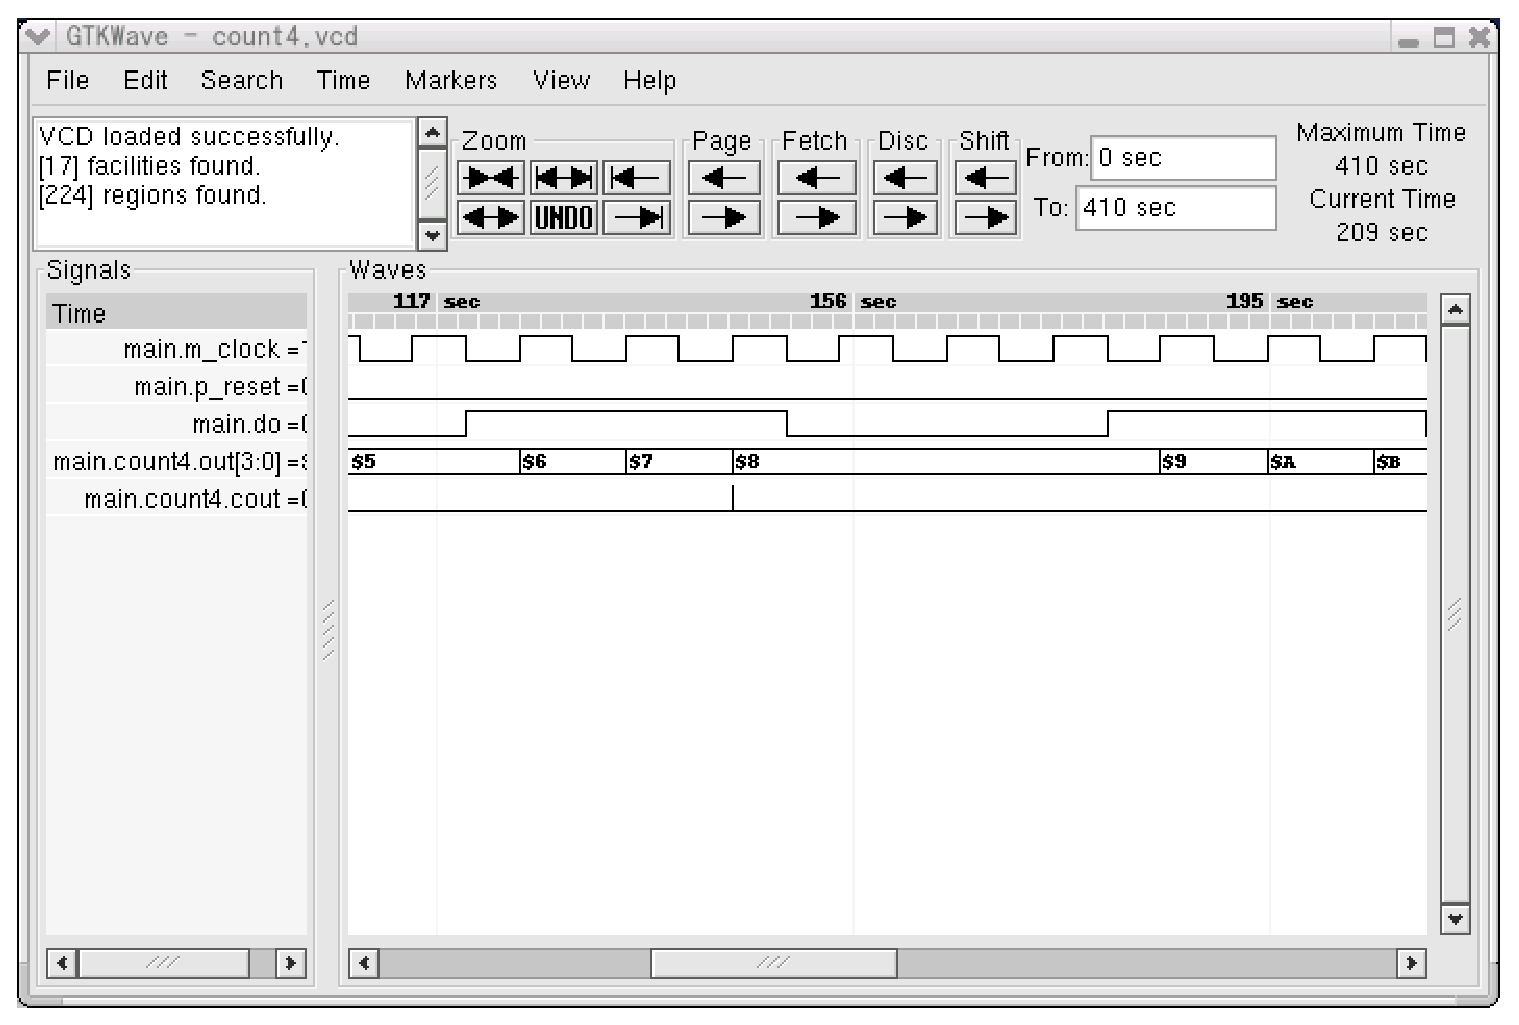
\includegraphics[scale=0.5]{count4_gtkwave.eps}
\caption{4ビットカウンタをシミュレーションした際の信号波形}
\label{fig:4ビットカウンタをシミュレーションした際の信号波形}
\end{center}
\end{figure}

\end{document}
%%% End of file (report.tex) %%%%%%%%%%%%%%%%%%%%%%%%%%%%%%%%%%%%%%%%%%%%%%
